\documentclass[tikz,border=10pt]{standalone}
\usepackage{tikz}
\usetikzlibrary{positioning,arrows.meta,shapes.geometric,fit,backgrounds,calc}

\begin{document}
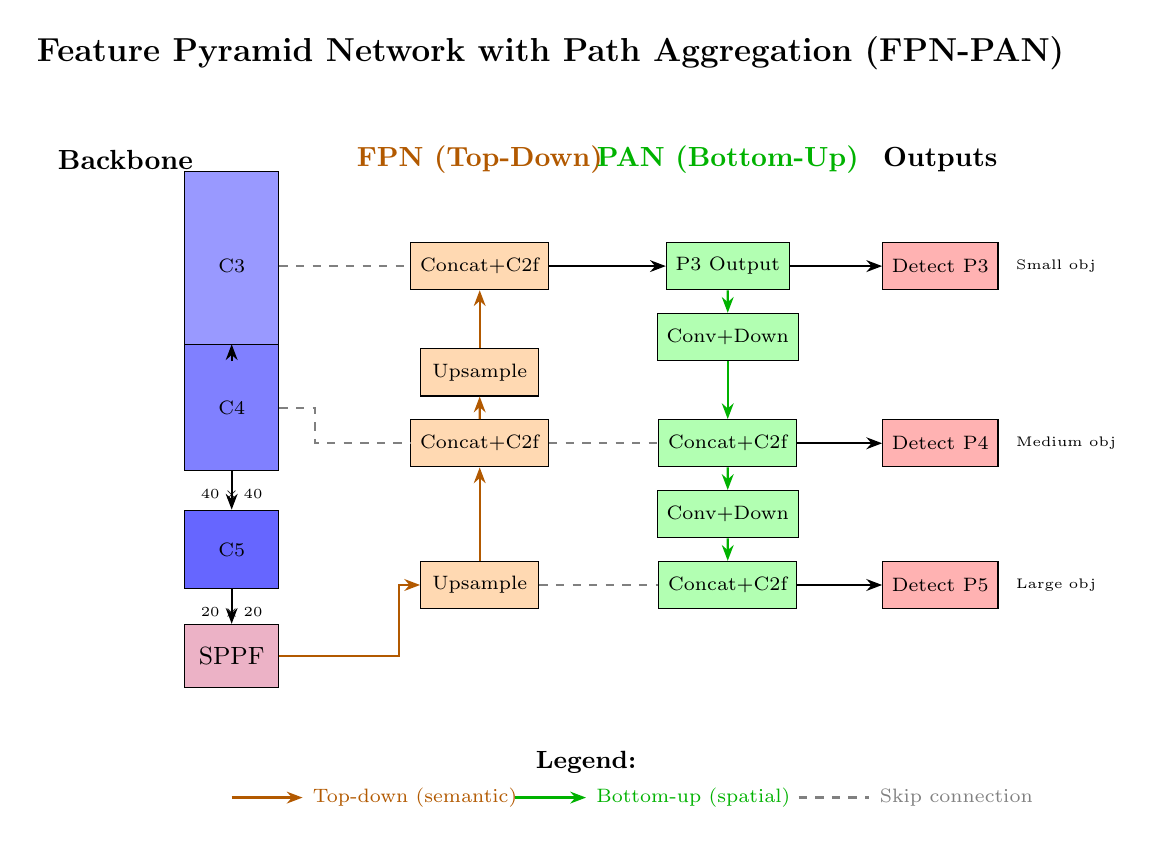
\begin{tikzpicture}[
    node distance=0.6cm and 1.5cm,
    scale=0.9,
    every node/.style={font=\small},
    featuremap/.style={rectangle, draw, minimum width=1.2cm, minimum height=#1, fill=blue!20},
    fpnblock/.style={rectangle, draw, fill=orange!30, minimum width=1.5cm, minimum height=0.6cm, font=\scriptsize},
    panblock/.style={rectangle, draw, fill=green!30, minimum width=1.5cm, minimum height=0.6cm, font=\scriptsize},
    arrow/.style={-{Stealth[length=2mm]}, thick},
    uparrow/.style={-{Stealth[length=2mm]}, thick, color=orange!70!black},
    downarrow/.style={-{Stealth[length=2mm]}, thick, color=green!70!black},
    skipline/.style={thick, dashed, color=gray}
]

% Title
\node[font=\bfseries\large] at (4.5,5) {Feature Pyramid Network with Path Aggregation (FPN-PAN)};

% Backbone feature maps (left side)
\node[font=\bfseries] at (-1.5,3.5) {Backbone};

% C3 - largest feature map (80x80)
\node[featuremap=2.4cm, fill=blue!40] (c3) at (0,2) {};
\node[font=\scriptsize] at (0,2) {C3};
\node[font=\tiny, below=0.1cm of c3] {$80 \times 80$};

% C4 - medium feature map (40x40)
\node[featuremap=1.6cm, fill=blue!50] (c4) at (0,0) {};
\node[font=\scriptsize] at (0,0) {C4};
\node[font=\tiny, below=0.1cm of c4] {$40 \times 40$};

% C5 - smallest feature map (20x20)
\node[featuremap=1cm, fill=blue!60] (c5) at (0,-2) {};
\node[font=\scriptsize] at (0,-2) {C5};
\node[font=\tiny, below=0.1cm of c5] {$20 \times 20$};

% SPPF
\node[rectangle, draw, fill=purple!30, minimum width=1.2cm, minimum height=0.8cm] (sppf) at (0,-3.5) {SPPF};

% FPN path (top-down) - middle column
\node[font=\bfseries, color=orange!70!black] at (3.5,3.5) {FPN (Top-Down)};

\node[fpnblock] (fpn5) at (3.5,-2.5) {Upsample};
\node[fpnblock] (fpn4) at (3.5,-0.5) {Concat+C2f};
\node[fpnblock] (fpn4up) at (3.5,0.5) {Upsample};
\node[fpnblock] (fpn3) at (3.5,2) {Concat+C2f};

% PAN path (bottom-up) - right column
\node[font=\bfseries, color=green!70!black] at (7,3.5) {PAN (Bottom-Up)};

\node[panblock] (pan3) at (7,2) {P3 Output};
\node[panblock] (pan3down) at (7,1) {Conv+Down};
\node[panblock] (pan4) at (7,-0.5) {Concat+C2f};
\node[panblock] (pan4down) at (7,-1.5) {Conv+Down};
\node[panblock] (pan5) at (7,-2.5) {Concat+C2f};

% Detection heads (rightmost)
\node[font=\bfseries] at (10,3.5) {Outputs};
\node[rectangle, draw, fill=red!30, minimum width=1.3cm, minimum height=0.6cm, font=\scriptsize] (head3) at (10,2) {Detect P3};
\node[rectangle, draw, fill=red!30, minimum width=1.3cm, minimum height=0.6cm, font=\scriptsize] (head4) at (10,-0.5) {Detect P4};
\node[rectangle, draw, fill=red!30, minimum width=1.3cm, minimum height=0.6cm, font=\scriptsize] (head5) at (10,-2.5) {Detect P5};

% Scale labels
\node[font=\tiny, right=0.1cm of head3] {Small obj};
\node[font=\tiny, right=0.1cm of head4] {Medium obj};
\node[font=\tiny, right=0.1cm of head5] {Large obj};

% Backbone arrows
\draw[arrow] (c3) -- (c4);
\draw[arrow] (c4) -- (c5);
\draw[arrow] (c5) -- (sppf);

% FPN arrows (top-down path)
\draw[uparrow] (sppf.east) -| ($(fpn5.west)-(0.3,0)$) -- (fpn5.west);
\draw[uparrow] (fpn5) -- (fpn4);
\draw[uparrow] (fpn4) -- (fpn4up);
\draw[uparrow] (fpn4up) -- (fpn3);

% Skip connections from backbone to FPN
\draw[skipline] (c4.east) -- ++(0.5,0) |- (fpn4.west);
\draw[skipline] (c3.east) -- ++(0.8,0) |- (fpn3.west);

% FPN to PAN arrows
\draw[arrow] (fpn3.east) -- (pan3.west);
\draw[downarrow] (pan3) -- (pan3down);
\draw[downarrow] (pan3down) -- (pan4);

% Skip connection from FPN to PAN
\draw[skipline] (fpn4.east) -- ++(0.5,0) |- (pan4.west);

\draw[downarrow] (pan4) -- (pan4down);
\draw[downarrow] (pan4down) -- (pan5);

% Skip connection from SPPF area to PAN5
\draw[skipline] (fpn5.east) -- ++(0.5,0) |- (pan5.west);

% Output arrows
\draw[arrow] (pan3.east) -- (head3.west);
\draw[arrow] (pan4.east) -- (head4.west);
\draw[arrow] (pan5.east) -- (head5.west);

% Legend
\begin{scope}[shift={(0,-5.5)}]
\node[font=\bfseries\small] at (5,0.5) {Legend:};
\draw[uparrow] (0,0) -- (1,0) node[right, font=\scriptsize] {Top-down (semantic)};
\draw[downarrow] (4,0) -- (5,0) node[right, font=\scriptsize] {Bottom-up (spatial)};
\draw[skipline] (8,0) -- (9,0) node[right, font=\scriptsize] {Skip connection};
\end{scope}

\end{tikzpicture}
\end{document}
